\documentclass[svgnames,11pt]{standalone}
\usepackage[utf8]{inputenc}
\usepackage[T1]{fontenc}
\usepackage{csquotes}
\usepackage[english]{babel}
\usepackage{xcolor}
\usepackage{charter}
\usepackage{amsmath}
\usepackage{amssymb}
\usepackage[np,autolanguage]{numprint}
\newcommand{\outqt}[1]{{\textcolor{DarkOrange}{#1}}}
\newcommand{\inqt}[1]{{\textcolor{Blue}{#1}}}
\usepackage{tikz}
\usetikzlibrary{arrows,automata,calc}
\usetikzlibrary{arrows.meta}
\usetikzlibrary{decorations.pathreplacing}
\usetikzlibrary{backgrounds,shapes}
\tikzset{%
  show curve controls/.style={
    postaction={
      decoration={
        show path construction,
        curveto code={
          \draw [blue] 
            (\tikzinputsegmentfirst) -- (\tikzinputsegmentsupporta)
            (\tikzinputsegmentlast) -- (\tikzinputsegmentsupportb);
          \fill [red, opacity=0.5] 
            (\tikzinputsegmentsupporta) circle [radius=.25ex]
            (\tikzinputsegmentsupportb) circle [radius=.25ex];
        }
      },
      decorate
}}}
\tikzstyle{vertex}=[draw,circle,black,inner sep=2pt]
\tikzstyle{edge}=[line width=1.3pt,color=Black]
\tikzstyle{rare}=[fill=black,text=white]
\tikzstyle{medium}=[fill=black!15!white]


\begin{document}
       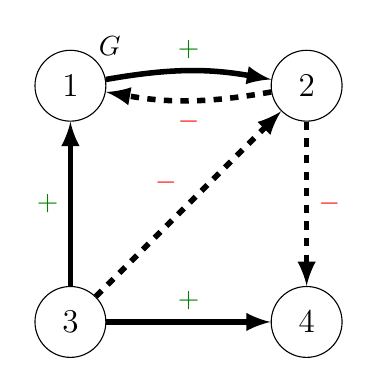
\begin{tikzpicture}[auto, every node/.style={transform shape},baseline=(b.base)]
         \tikzset{>=latex}
         \tikzstyle{peers}=[draw,circle,black,minimum width=9mm,inner sep=2pt]
         \tikzstyle{nedge}=[draw,rectangle,black,minimum width=8.5mm,minimum height=8.5mm, inner sep=0]
         \tikzstyle{edge}=[line width=2pt,color=Black,->]
         \tikzstyle{uedge}=[line width=2pt,color=Black]
         \tikzstyle{pnode}=[fill=White]
         \tikzstyle{elabel}=[color=Black]
         \tikzstyle{qnode}=[fill=White]
         \tikzstyle{posc}=[color=Green]
         \tikzstyle{negc}=[color=red]
         \foreach \place/\name in { {(0,0)/1}, {(3,0)/2}, {(0,-3)/3}, {(3,-3)/4}}
         \node[peers,pnode] (\name) at \place {\large $\name$};
         \draw[edge] (3) -- node [posc]                            {$+$}  (1);
         \draw[edge] (3) -- node [posc]                           {$+$}  (4);
         \draw[edge, dashed] (3) -- node [negc]                    {$-$}  (2);
         \draw[edge, dashed] (2) -- node [negc]                    {$-$}  (4);
         \draw[edge] (1) edge [bend left =10] node [posc]         {$+$} (2);
         \draw[edge, dashed] (2) edge [bend left =10] node [negc] {$-$} (1);
         \node[] (caption) at (0.5, 0.5) {$G$};
         \node[] (b) at (1.5, -1.5) {};
       \end{tikzpicture}
\end{document}
